
\subsection{Summary}

This paper reports the successful reproduction of the results in a
paper I co-authored in 2008\supercite{Eglen2008-ca}. A postprint of
this paper is available at
\url{https://arxiv.org/abs/1208.0986}. (Open access was not mandated
by the funders of this research at the time of publication.) All the
code has been uploaded to \url{https://github.com/sje30/rescience-hor}
along with the Rmarkdown sources for this report.

\section{Historical context}


\subsection{Scientific question}

To investigate a problem in neurobiology concerning the relative spatial
positioning of two types of neuron in the retina. We used three example
datasets (pretty much all that was available at the time) to investigate
this problem using spatial statistics and simulations of spatial
patterning. These datasets were not available in digital format, but the
images\supercite{Wassle1978-cd,Wassle2000-aa} were
scanned in and digitised (each cell represented as an x,y location) by
me as part of the work for the original paper. These datasets were not
publicly shared before.

\subsection{Computational context}

Most of the code required for the 2008 paper had been developed by
myself since about 2000 working on other related problems. The major
innovation here was in the biological problem.

One of the key reasons I switched to R as a programming environment in
the late 1990s was because of the strong support it had for spatial
statistics. In particular the SPLANCS
package\supercite{splancs} in R has been a key package in most of my research.

\subsection{Original source code}

the original source code was not published or publicly archived before.
The source code was kept just on my hard drive. I keep good backups
though, and in this case the projects were still in my home directory
(copied from machine to machine over the years). No license was written
systematically to cover the code I wrote, although the R packages are
usually released under GPL or MIT.

As a side-effect of producing this article, the following R packages of
mine were made available:

\begin{enumerate}
\item
  sjedmin: dmin model for spatial point patterns.
  \url{https://github.com/sje30/sjedmin}
\item
  sjedist: unified calculation of spatial statistics.
  \url{https://github.com/sje30/sjedist}
\item
  sjevor: Wrapper around public domain code for Voronoi tessellation
  \url{https://github.com/sje30/sjevor}
\end{enumerate}

The Voronoi tessellation was public domain C code provided by Steve
Fortune\supercite{Fortune1987-kg}. (This code was not required for the current
project, but was implicitly required for the parent package, sjedist.)

\subsection{Retrieval of the software}

This was relatively straightforward, as the software was all on my hard
drive. One complication was that until a few years ago, I had been using
RCS as my primary version control software. As I wished to release the
packages onto github, I converted the history from RCS into Git using
the tool \texttt{https://github.com/Oblomov/rcs-fast-export}.

I anticipated that loading the data might be tricky, as I had used R's
internal Rda format to efficiently store the data files (they are not
large, so there was no need to be concerned about efficiency). Given
that this format could in principle change over time, this might have
been a problem. However, R 4.0.0 was able to read in the file
\texttt{bivariate\_mosaics.Rda}.

\section{Execution}

The code ran fine in today's version of R (4.0.0); see end of document
for the full list of R dependencies. I did not need to load any older
versions of libraries. The code was tested on both my laptop (ThinkPad
T480s running Manjaro linux) and on \url{https://mybinder.org} (see the
end of this document for mybinder details.) The simulations themselves
only take a couple of minutes to run. If recompiling on binder, it takes
a few more minutes to install all the packages and initialise the tex
distribution.

However, although the code worked fine, it took me about 20 minutes to
read through the old scripts and work out what to do, as I had not
provided a Makefile or similar.

Once the code was running, I only wished to make cosmetic updates to the
project to modernise it. The most significant change was converting the
format for figures from postscript to pdf as there is more support for
the latter. The three figures that were generated are reproduced in this
paper and can be compared against the figures from the original paper.

A Makefile is provided to help regenerate the simulation results and the
figures. \emph{make clean} will return the repository to a clean state.
\emph{make all} will first run the simulations and store the results in
several \emph{.Rda} files. There are then several R scripts to generate
the figures from the corresponding \emph{.Rda} files. Finally, after the
figure pdfs have been generated, this document is compiled from its
Rmarkdown source.

\subsection{Retrieval of the software}

This was relatively straightforward, as the software was all on my hard
drive. One complication was that until a few years ago, I had been using
RCS as my primary version control software. As I wished to release the
packages onto github, I converted the history from RCS into Git using
the tool \texttt{https://github.com/Oblomov/rcs-fast-export}.

I anticipated that loading the data might be tricky, as I had used R's
internal Rda format to efficiently store the data files (they are not
large, so there was no need to be concerned about efficiency). Given
that this format could in principle change over time, this might have
been a problem. However, R 4.0.0 was able to read in the file
\texttt{bivariate\_mosaics.Rda}.

\section{Execution}

The code ran fine in today's version of R (4.0.0); see end of document
for the full list of R dependencies. I did not need to load any older
versions of libraries. The code was tested on both my laptop (ThinkPad
T480s running Manjaro linux) and on \url{https://mybinder.org} (see the
end of this document for mybinder details.) The simulations themselves
only take a couple of minutes to run. If recompiling on binder, it takes
a few more minutes to install all the packages and initialise the tex
distribution.

However, although the code worked fine, it took me about 20 minutes to
read through the old scripts and work out what to do, as I had not
provided a Makefile or similar.

Once the code was running, I only wished to make cosmetic updates to the
project to modernise it. The most significant change was converting the
format for figures from postscript to pdf as there is more support for
the latter. The three figures that were generated are reproduced in this
paper and can be compared against the figures from the original paper.

A Makefile is provided to help regenerate the simulation results and the
figures. \emph{make clean} will return the repository to a clean state.
\emph{make all} will first run the simulations and store the results in
several \emph{.Rda} files. There are then several R scripts to generate
the figures from the corresponding \emph{.Rda} files. Finally, after the
figure pdfs have been generated, this document is compiled from its
Rmarkdown source.


\subsection{Reproduction of results}

The results generated closely matched those that were presented in the
original paper. As the simulation methods are stochastic (and no seed
was set for reproducible random number generation), the P values
reported in Figure 2 do not match those originally reported, nor does
the simulation field (right hand side of Figure 1) match. However, the
statistical properties of the models still match those of the
experimental data.

\subsection{Could someone else reproduce the work?}

If I had simply given the R code and packages to someone else, the lack
of documentation or Makefile would have meant that this person would
have needed to study the code carefully to work out what files were
generated. I would have hoped though that someone fluent with R would
have made sense of the code itself, and all of the parameters for the
simulations were included in the source files.

\section{Reproduction of Figure 1}

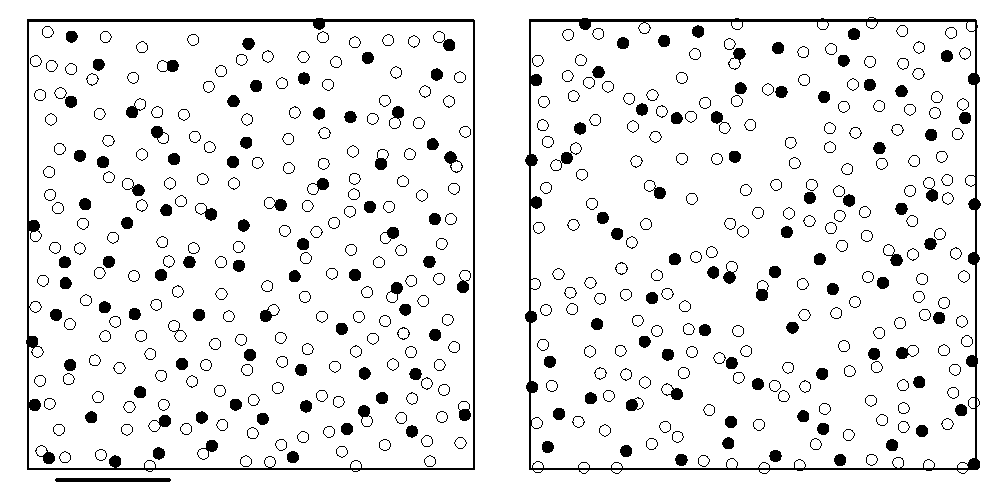
\includegraphics[width=\textwidth]{../hor_fieldA_col.pdf}

We also made a supplementary figure of all 3 fields.

\section{Reproduction of Figure 2}

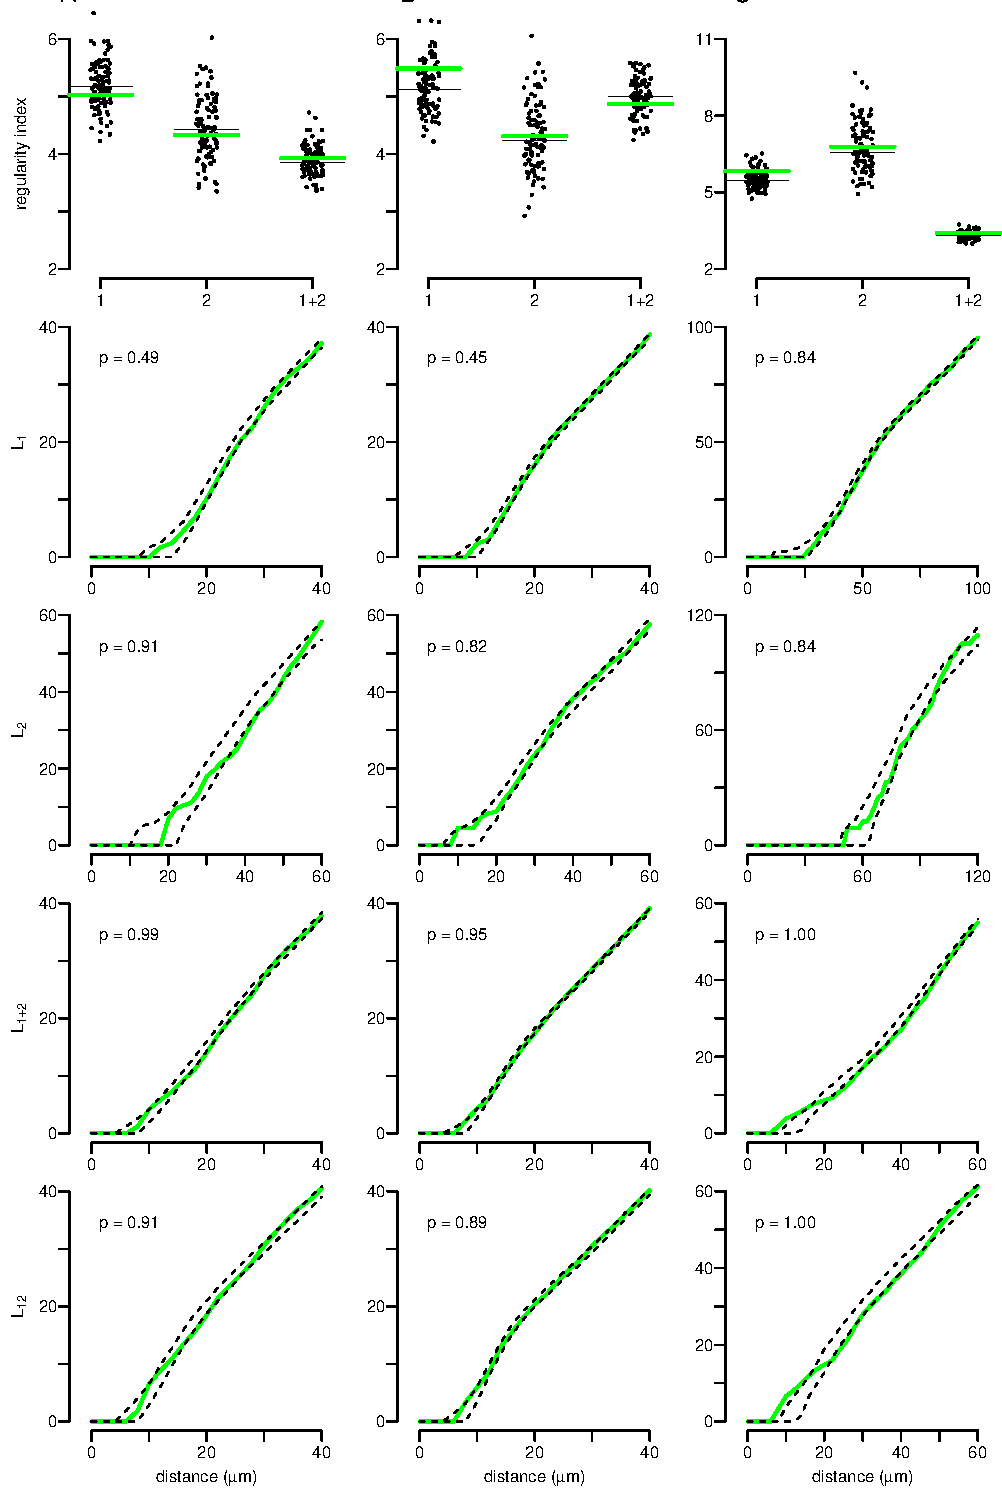
\includegraphics[width=\textwidth]{../eglen_fig2_col.pdf}

\section{Reproduction of Figure 3}

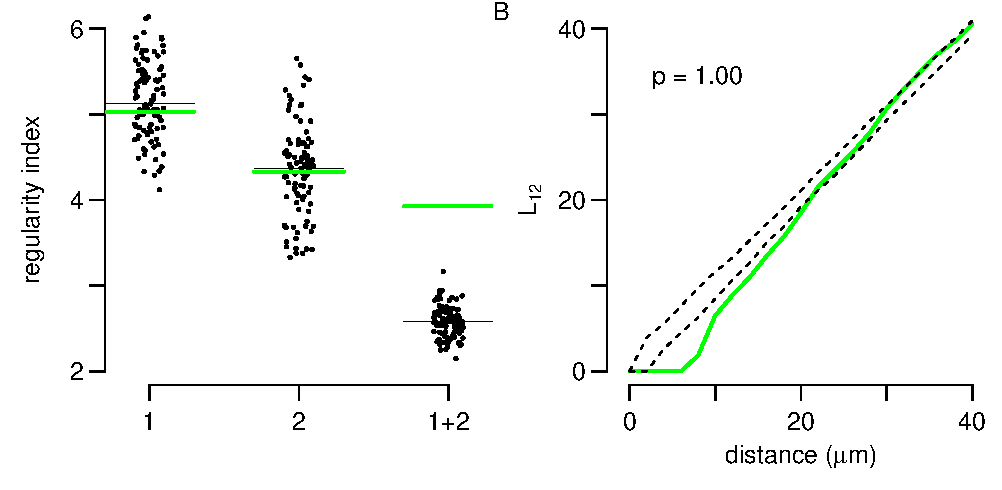
\includegraphics[width=\textwidth]{../eglen_fig3_col.pdf}

\hypertarget{reproduction-of-table-2}{%
\section{Reproduction of Table 2}\label{reproduction-of-table-2}}

Key column from table 2 is the rejects column which is reproduced in
Table~\ref{tab:rep}.  The other columns of this table were determined
statically from the data sets, so were not recalculated here.  (Had I
known more about generating tables in R at the time, I think my R code
should have created this entire table.)


\begin{table}[h!]
  \centering
  \begin{tabular}{llll}
    \hline
    field & rejects & n$_{\mathrm{pairs}}$ & rejects / n$_{\mathrm{pairs}}$ \\ \hline
    C & $242 \pm 10$ & 25500 & 0.01\\
    A & $937 \pm 36$ & 15334 & 0.06\\
    B & $7202 \pm 300$ & 17716 & 0.41\\
    \hline
  \end{tabular}
  \caption{Reproduction of table 2 results}
  \label{tab:rep}
\end{table}

%% copied from table2-rejects.txt


\section{Conclusions}

It was relatively easy to recompute the results in this report, because
of the stability of the R environment and its packaging system. Even its
binary data format (.Rda) for storing objects was reusable over a 10
year timescale. The largest challenge was the user issue of remembering
what I had done to run the analysis and generate the results. Using
mybinder.org was useful to iron out minor issues that others might face
trying to run the software on their machine. In its current state, the
repository requires R and make -- if make is unavailable, the scripts
would need to be run by hand, which is not onerous, but writing them out
explicitly might help those unfamiliar with Make syntax.

